\part{Contexte}
\chapter{L'entreprise}
\section{Alter Way}
\paragraph*{}
	Alter Way est une entreprise spécialisée dans les services informatiques utilisant des logiciels open source
	\footnote{Un logiciel open source est un logiciel dont le code source est librement accessible et modifiable par tout le monde.}.
	Elle est composée de cinq groupes afin de répondre à l'ensemble des besoins des SI\footnote{Système d'Information}:
	\begin{description}
		\item[Hosting] Hébergement et infogérance système de site web
		\item[Solution] Développent, maintenance et infogérance applicatif de site web
		\item[Formation] Formation standard, cursus de formation, coatching
		\item[Consulting] Conseil, audit, industrialisation
		\item[Creative] Conseil en communication, infographisme
	\end{description}

	\begin{figure}
	\centering
	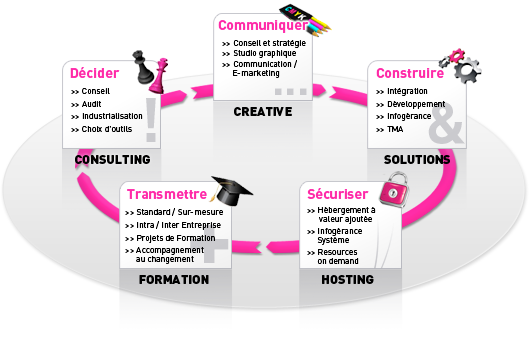
\includegraphics[width=0.9\textwidth]{resource/img/aw_360}
	\caption{Les différentes branches d'Alter Way}
	\end{figure}

\section{Histoire}
\paragraph*{}
	Créee en 2006, Alter Way est la première entreprise française à avoir fédéré les acteurs historique
	de l'open source autour d'un projet d'industrialisation du marché:

	\begin{description}
		\item[Anaska] Leader français de formation open source en 2001
		\item[Eclip's Software] Éditeur d'une solution d'administration réseau
		\item[Ingeniweb] Spécialiste en solution web d'entreprise de gestion de contenu
		\item[Kanopee] Consultants en développement PHP
		\item[Nexen Services] Hébergement et Infogérance LAMP\footnote{Linux Apache MySQL PHP}
		\item[O4DB] Expertise en BDD\footnote{Base de Donnée}
		\item[Solinux] Spécialistes dans l'administration de platforme Linux et l'intégration d'OpenXchange
	\end{description}

	Afin de renforcer son offre globale et de soutenir sa stratégie de développement sur le web, Alter Way
	a également intégré l'agence de communication \emph{Reciprok}, spécialisée en conseil en communication,
	studio graphique et web-marketing.

	\begin{figure}
		\centering
		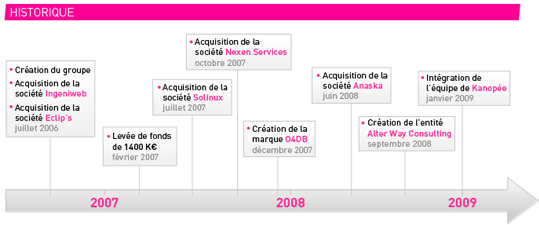
\includegraphics[width=0.9\textwidth]{resource/img/historique_aw}
		\caption{L'histoire d'Alter Way}
	\end{figure}

\section{Quelques chiffres (2010)}
	\begin{itemize}
		\item 10M\euro{} de Chiffre d'affaire
		\item 10\% de croissance
		\item Résultats: +4.5\%
		\item 120 collaborateurs
	\end{itemize}

\section{Alter Way Hosting}
\paragraph*{}
Alter Way Hosting (AWH), anciennement Nexen Services est la branche de la société dont le rôle est l'hébergement et l'infogérance de services internet.
Les services hébergés sont pour la plupart des sites web ainsi que des serveurs de messagerie.

\paragraph*{}
AWH est organisé en quatres équipes affectées à quatres types d'offres différentes:

\begin{description}
	\item[L'équipe responsable des serveurs dédiées vserveurs \footnotemark]
		\footnotetext{Technologie de virtualisation de système d'exploitation permettant d'héberger plusieurs clients sur un seul serveur}
	\item[L'équipe responsable des offres mutualisées
		\footnotemark] \footnotetext{Plusieurs sites internet sont hébergés sur un même serveur par un seul logiciel de serveur web}
	\item[Les RTC \footnotemark des architectures] \footnotetext{RTC: Responsable Chef de Compte, similaire à Chef de Projet}
		gèrent les clients les plus importants possédant plusieurs serveurs dédiés
	\item[Les responsable de l'infrastructure] s'occupent des tâches plus globale touchant à tout les serveurs,
		principalement la gestion du réseau.

\end{description}


\section{Hiérarchie}

\begin{figure}[H]
	\centering
	\includegraphics[width=1\textwidth]{resource/graph/hier}
	\caption{La hiérarchie d'Alter Way}
\end{figure}

\chapter{Sujet du stage}

\section{Contexte Technologique}

\section{La virtualisation}
\label{virtualisation}
\paragraph*{}
La virtualisation consiste à faire fonctionner un logiciel ou un système d'exploitation (SE) dans un environnement simulé/virtuel.
\\
Normalement un logiciel est éxécutée par le processeur (CPU) de l'ordinateur. Dans le cas de la virtualisation au niveau logiciel,
ce logiciel ne sera pas éxécuté directement par un vrai CPU mais par un autre logiciel appelé gestionnaire de machine virtuelle.
\\
Dans le cas de la virtualisation d'un OS (appelé virtualisation matérielle, plusieurs solutions sont possible. La solution la plus basique est de simuler l'intégralité
de l'ordinateur: le CPU, le disque dur, la carte réseau, l'écran, la souris, le clavier ect.
Il devient alors possible de faire fonctionner un OS ou plusieurs OS dans un autre OS.

\subsection{La virtualisation de système d'exploitation}
\label{virtualisation_mat}
\subsubsection{Les différentes techniques}
\paragraph*{}
Il existe plusieurs méthode pour virtualiser un système d'exploitation. Chacunes d'elles ont des avantages et des
inconvéniants. Le choix d'une méthode est un compromis entre les performances, l'isolation des systèmes virtualisés,
et la simplicité de mise en oeuvre.

\paragraph*{}
Dans ce document, nous appelerons les systèmes d'exploitations virtualisés/invités \textbf{VM} comme \emph{Virtual Machine} ou \textbf{domU} suivant le contexte.
Le système d'exploitation principal/hôte sera appelé dom0 ou hyperviseur si aucun autre logiciel n'a déjà ce role dans l'architecture de virtualisation
utilisée.

\paragraph*{}
\begin{description}

	\item[Par émulation] Fig \ref{emulation} : Relativement facile à mettre en oeuvre, compatible avec tout les systèmes d'exploitations et toutes les architectures
	de processeur.\\
	L'isolation des VMs est parfaite mais les performances sont extrêmement mauvaises.

	\item[Par isolation] Fig \ref{isolation} : Moyennement facile mettre en ouvre, oblige à avoir exactement le même système d'exploitation dans le domU et le dom0.\\
	L'isolation des VMs est généralement très faible mais les performances sont maximal. Les VMs se partagent de manière optimale les ressources de la machine.

	\item[Par noyau en espace utilisateur] Fig \ref{userkernel} : Moyennement facile à mettre en oeuvre et ne fonctionne qu'avec le système d'exploitation Linux en domU.\\
	L'isolation des VMs est très bonne mais les performances plutôt mauvaises.

	\item[Par hyperviseur] Fig \ref{hypervisor} : Un peu complexe à mettre en oeuvre mais est capable d'avoir de très bonnes performances si le système d'exploitation invité
	utilise des drivers spéciaux pour fonctionner de manière optimisée avec l'hyperviseur.\\
	L'isolation est aussi bonne que la méthode par émulation. Si l'OS invité ne contient pas les bons drivers, la VM marchera tout de même mais
	avec des performances dégradées.

\end{description}

\begin{figure}[H]
\centering
\subfloat[Par émulation]{\label{emulation}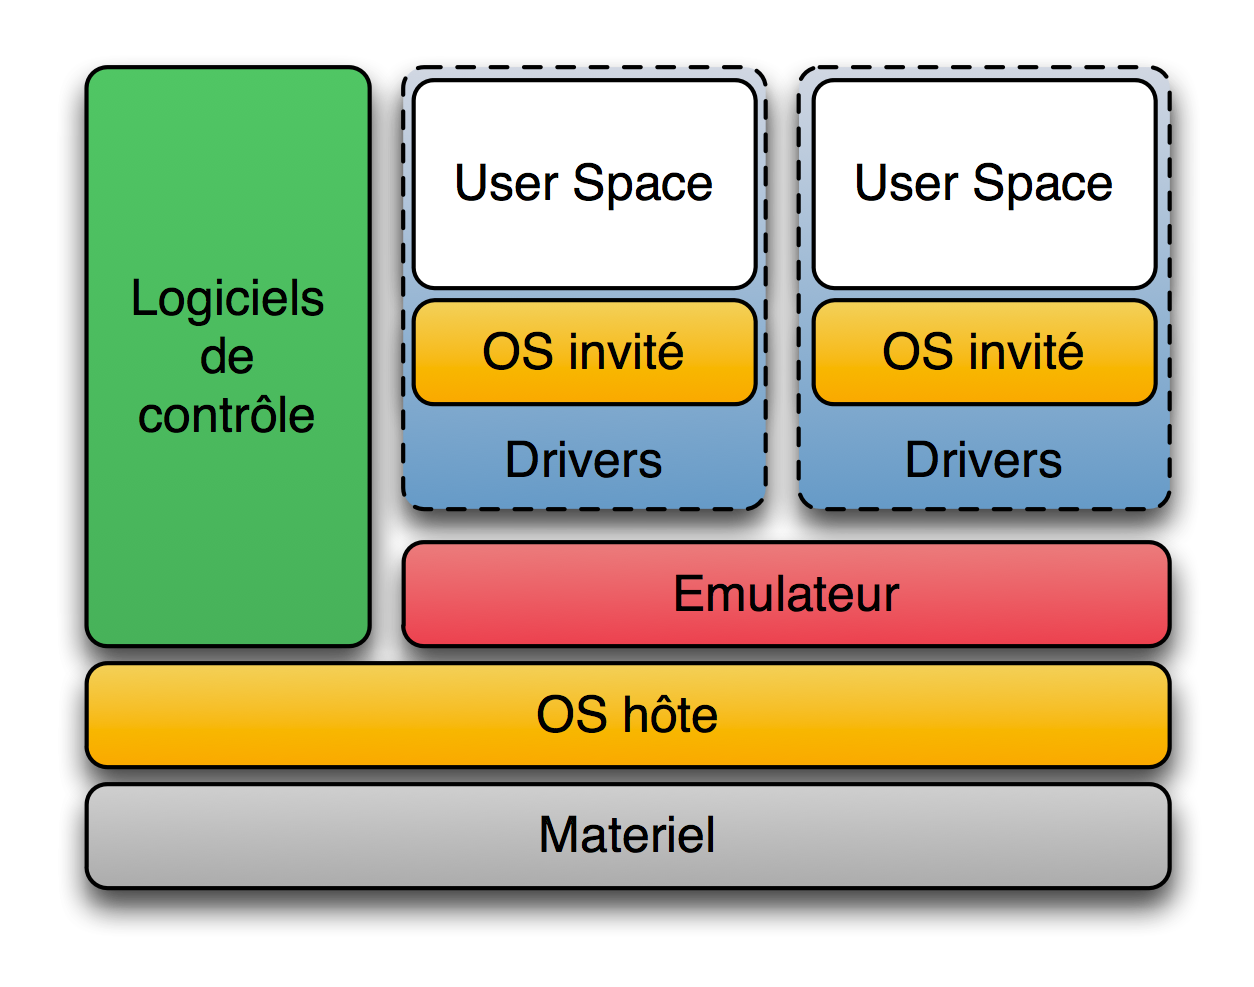
\includegraphics[width=0.4\textwidth]{resource/img/Diagramme_ArchiEmulateur}}
\subfloat[Par isolation]{\label{isolation}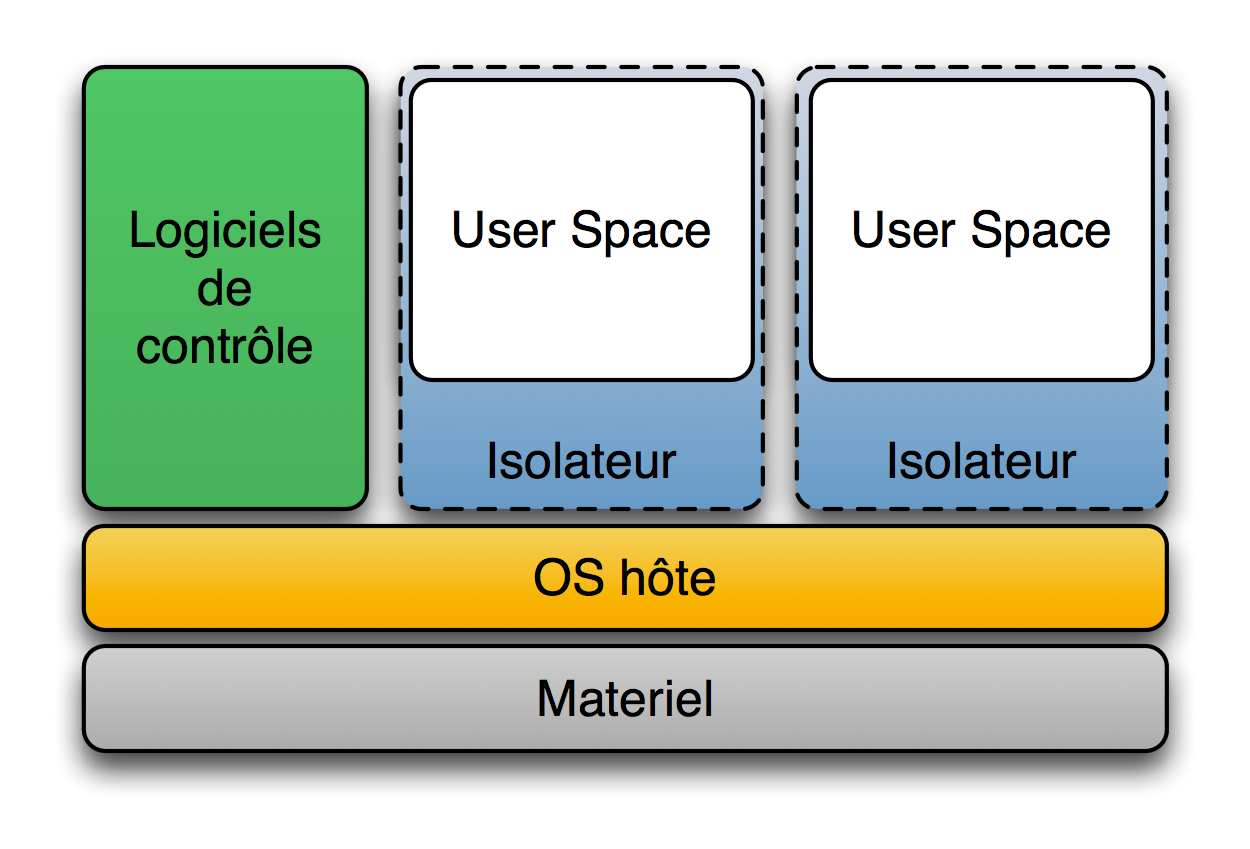
\includegraphics[width=0.4\textwidth]{resource/img/Diagramme_ArchiIsolateur}}
\\
\subfloat[Par noyau en espace utilisateur]{\label{userkernel}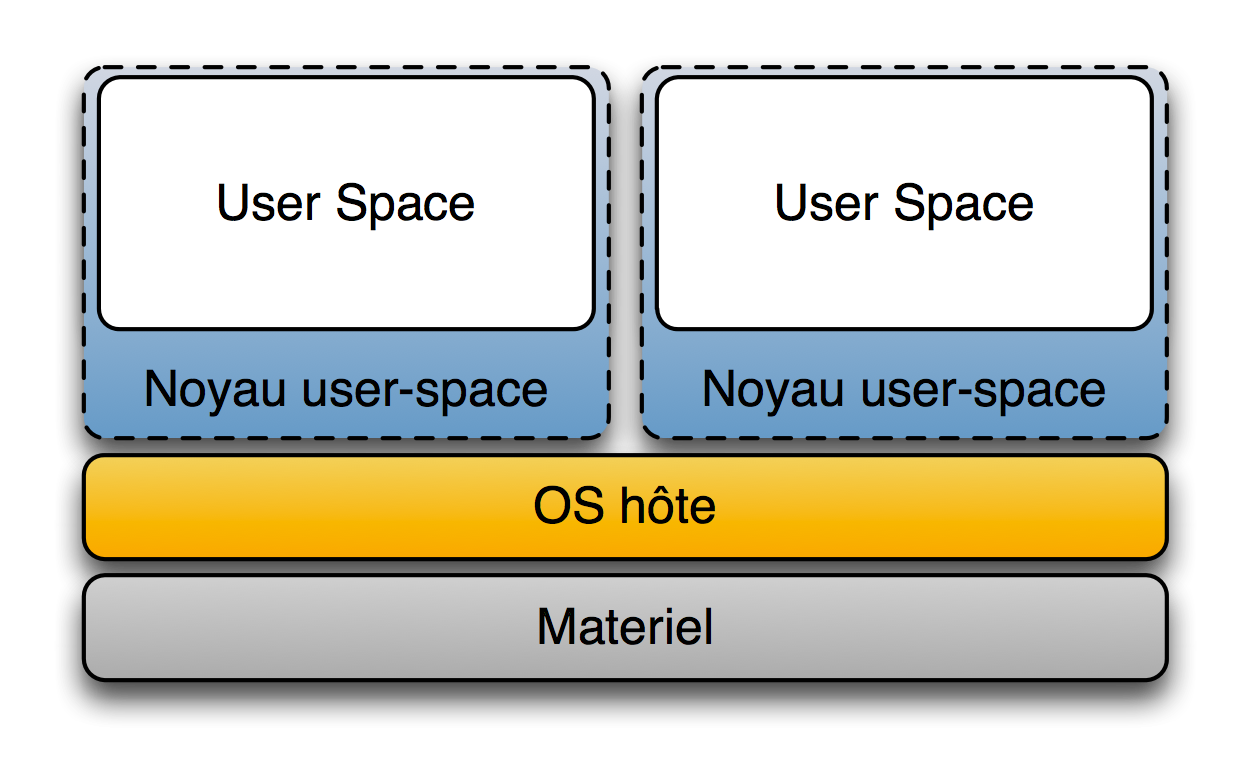
\includegraphics[width=0.4\textwidth]{resource/img/Diagramme_ArchiKernelUserSpace}}
\subfloat[Par hyperviseur]{\label{hypervisor}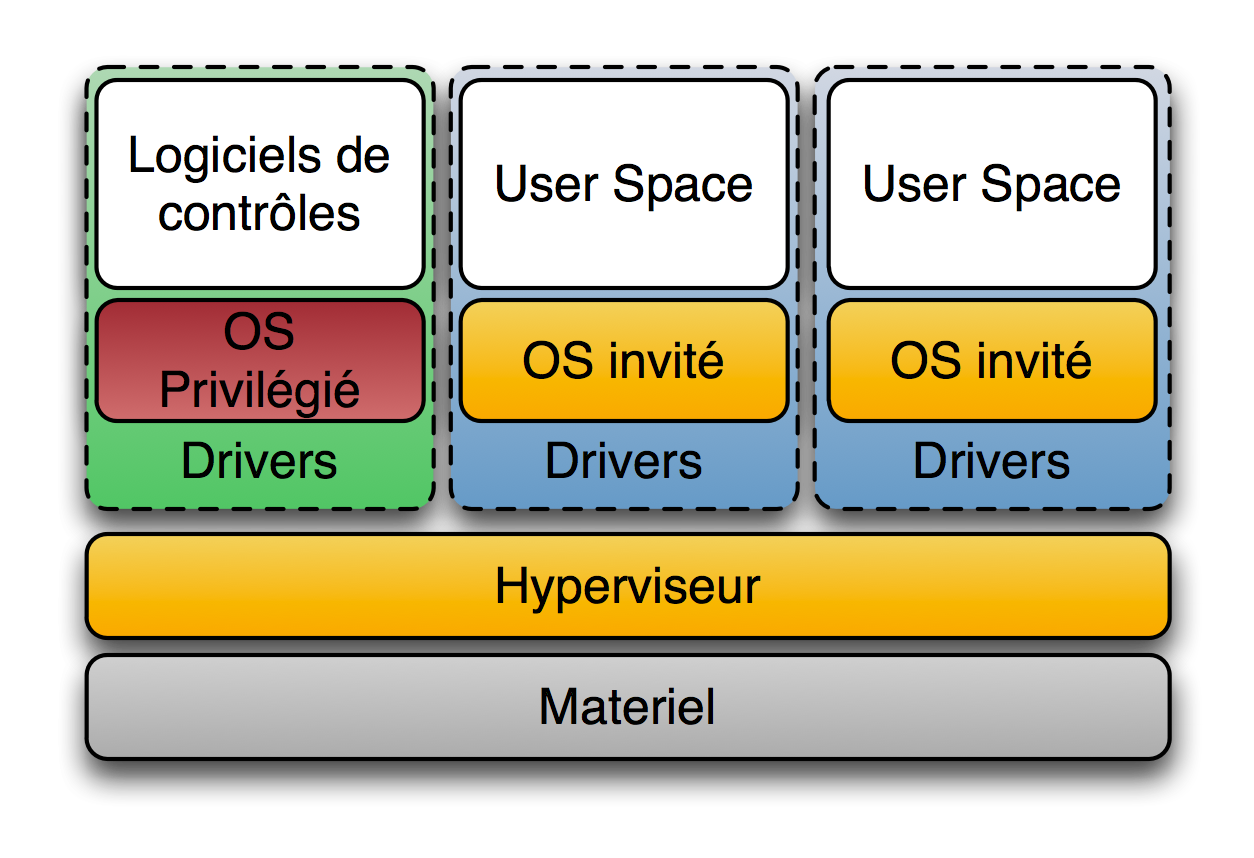
\includegraphics[width=0.4\textwidth]{resource/img/Diagramme_ArchiHyperviseur}}
\caption{Les différentes architectures de virtualisation d'OS}
\end{figure}


\section{Le cloud computing\index{Cloud Computing}}
\label{cloud}
\subsection{Principe général}
\paragraph*{}
Le \emph{cloud computing} \footnote{Litéralement: "informatique dans les nuages"} est expression
très à la mode ces dernières années et possède une définission très large.
Le principe général est d'externaliser sur des serveurs distants des données ou
des traitements informatiques.

\paragraph*{}
L'avantage pour l'utilisateur du service est qu'il n'a plus à ce soucier d'où se situent physiquement
ses données ni de l'administration des serveurs. Toutes les contraintes de sécurité, de disponibilité
et de fiabilité sont déportées à la responsabilité de l'hébergeur.

\paragraph*{}
Pour l'hébergeur, les avantages sont aussi certain: Le cloud computing permet de mutualiser au maximum
les infrastructures matériels et d'industrialiser une grande partie des processus d'administration.
Par conséquence cette technique permet de diminuer sensiblement les coûts et/ou d'augmenter la qualité
de service.

\subsection{Les différents types de Cloud}

\subsubsection{SaaS\index{SaaS: Software as a Service}}
\paragraph*{}
Le principe du Saas consiste le plus souvent à fournir un service sous la forme d'une application web.
Le type de service rendu est traditionnelement celui que pourrait fournir une application classique.
\\
L'exemple le plus populaire est le webmail\footnote{Interface client de gestion de mail sous forme d'un site web}, comme GMail de Google.

\paragraph*{}
La maintenance des serveurs, de leurs systèmes d'exploitation et des logiciels est faite par le fournisseur de service.
Pour le client, la maintenance ainsi que les MAJ\footnote{MAJ: Mise à jour} des logiciels est transparente et invisible.
\\
Par exemple, personne ne connait le numéro de version de GMail et ça n'interesse personne.

\subsubsection{PaaS\index{PaaS: Platform as a Service}}
\paragraph*{}
Le PaaS est similaire au Saas à la différence que la gestion du logiciel métier est assuré par le client.
Le fournisseur fournit les serveurs et s'occupe de la bonne configuration du système d'exploitation et des middleware
\footnote{Middleware: Logiciel n'étant pas utilisé directement par le client mais par le logiciel métier ou d'autres middlewares} afin
que le logiciel du client fonctionne convenablement.

\paragraph*{}
Alter Way Hosting, est un bon exemple de fournisseur de PaaS: \\
\begin{itemize}
\item 	Le client développe et maintient son site web puis le fournit à AWH.\\
\item 	AWH s'occupe d'acheter, de configurer et de brancher en Data Center\footnote{un Data Center, souvent abbrégé en DC, est une salle
		ou un batiment spécialisé pour y brancher des serveurs} les serveurs puis d'installer et configurer l'OS et les middlewares pour que
		le site web du client fonctionne correctement.
\end{itemize}

\subsubsection{IaaS\index{IaaS: Infrastructure as a Service}}
\paragraph*{}
Dans le cas de l'IaaS, le fournisseur de service, ne s'occupe plus que de founir du matériel au client: serveurs, stockage, réseau...
\\
Ce type d'offre est le plus souvent mise en place gràce à la virtualisation (voir chapitre \ref{virtualisation}) de système d'exploitation.
\\
L'entreprise Amazon, fût pionière dans le domaine de l'IaaS gràce à leur offre d'\textsl{Elastic Compute Cloud}: EC2.

\subsection*{} %To get correct spacement

\begin{figure}[H]
\centering
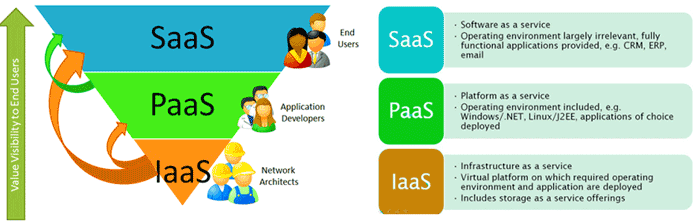
\includegraphics[width=0.9\textwidth]{resource/img/clouds-users}
\caption{Les différents utilisateur du Cloud}
\end{figure}

\begin{figure}[H]
\centering
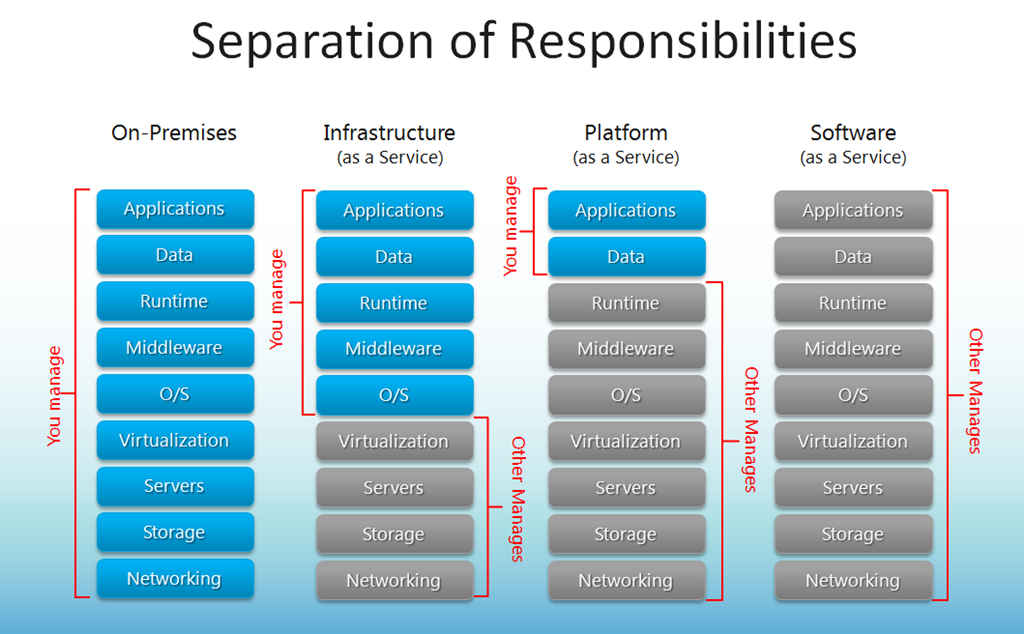
\includegraphics[width=0.9\textwidth]{resource/img/clouds-responsabilities}
\caption{Les différentes responsabilitées des acteurs du Cloud}
\end{figure}

\subsection{Le cloud appliqué à l'hébergement de services ou d'OS\protect\footnote{De l'anglais \textit{Operating System}: Système d'exploitation}}
\paragraph*{}
Le principe du cloud peux être appliqué au niveau du serveur physique et du système d'exploitation. Le responsabilité du fournisseur est de créer/préparer
à la demande du client des machines toutes prêtes avec un système d'exploitation et la bonne configuration réseau.

\paragraph*{}
Souvent, les machines créées ne sont pas des machines physiques mais des machines virtuelles. L'avantage de l'utilisation de machines virtuelles (VM), est
qu'il n'est plus nécéssaire de manipuler physiquement des équipements (serveurs, routeurs, NAS...).
\\
Il est donc possible d'automatiser et d'industrialiser le processus de création d'une nouvelle machine.
\\
Par exemple, sur le site d'amazon, il suffit d'entrer ses coordonnées bancaires et de renseigner quelques options (puissance de la machine, système d'exploitation, logiciels à préinstaller ...)
 pour avoir accès à une machine toute prête en quelques secondes seulement. Ensuite, via un simple clic, il est possible de changer le nombre de machine que l'on veux.
La facturation est calculé à la seconde. Ce type d'offre est donc très pratique pour les personnes ayant besoin de beaucoup de puissance durant un court laps de temps.

\section{La problématique d'Alter Way Hosting}

\paragraph*{}
Toute cette partie décris la étapes qui ont été réalisés en amont de mon arrivé dans l'entreprise.

\subsection{État actuel}
\paragraph*{}
Lorsqu'un client fait une demande de serveur, l'équipe doit:
\begin{itemize}
	\item Prendre un serveur dans le stock ou commander un.
	\item Le personnaliser en fonction des besoins du clients: Ajouter de la RAM, des disques, des processeurs ...
	\item Installer l'OS Debian dessus et le configurer
	\item Emmener et "racker"\footnote{Terme que l'on utilise pour désigner l'installation d'une lame de serveur dans un rack (baie informatique).\\
		Voir l'annexe \ref{rack}} le serveur
	dans le bon Data Center (DC).
	\item Configurer les équipements réseaux et vérifier que tout fonctionne bien.
\end{itemize}

Ce processus est long et laborieux et n'est pas très flexible. Il n'est pas possible sans intervention physique sur la machine d'augmenter ou diminier sa puissance.

\subsection{Cahier des charges}
\paragraph*{}
L'objectif d'Alter Way Hosting est d'industrialiser/automatiser le processus de deployement et de mise à jour des serveurs.

\paragraph*{}
Depuis quelques années, l'industrie de l'hébergement informatique est en train de migrer vers une structure de type Cloud utilisant la virtualisation.
Cela permet de faire abstraction des problématiques matérielles. Il devient possible de créer, détruire et même redimentionner des machines virtuelles en
quelques secondes via une simple interface de commande.

\subsubsection{Acteurs du projet}

Dans un premier temps, la nouvelle plateforme ne servira pas directement aux clients mais seulement aux techniciens s'occupent des
demandes des clients.\\
Les responsables clients sont des habitués de la ligne de commande et pourront se contenter d'une interface de controle simple mais par la suite
il faudrait que les clients ou les commerciaux puissent directement commander et régler en ligne leur commande.

\subsubsection{Fonctionnalités désirés}

\lipsum[1]

\subsection{Recherche de solutions}
\paragraph*{}
Un travail en amont réalisé par mon tuteur de stage a permis de déterminer une solution technique pour répondre aux besoins d'AlterWay.\\
Cet solution utilise comme logiciels l'hyperviseur de virtualisation \textbf{Xen} et le gestionnaire de Cloud \textbf{OpenNebula} et des
serveurs de stockage \textbf{NetApp}\footnote{NetApp est une société fabriquant des serveurs spécialisée dans le stockage reseau de type SAN (voir \ref{san})}.

\paragraph*{}
Lors de la recherche du logiciel de gestion de cloud, aucune solution ne correspondait entièrement à nos attentes. Les deux logiciels se rapprochant le plus
de nos objectifs étaient:
\begin{description}
	\item[OpenStack] est un logiciel open source créée par Rackspace et la NASA. Plus de 120 compagnies ont joint le projet dont Citrix System, Dell, AMD, Intel,
		Canonical, SUSE Linux, HP et Cisco.\\
		C'est le projet qui évolue probablement le plus vite et qui est le plus complet sur le plan des fonctionnalités.
	\item[OpenNebula] est un autre logiciel open source principalement financé par RESERVOIR
	\footnote{Une organisation européenne de financement de projet open source dans le domaine du Cloud Computing} et auquel contribue d'autres organisations
	comme l'INRIA, le CNRS et d'autres organisations et universités européennes.\\
	Ce logiciel est moins avancé cependant les fonctionnalités nous interessant qui sont absentes ne le sont pas non plus dans OpenStack.
\end{description}

\paragraph*{}
Aucune solution existante ne convenant parfaitement à notre besoin, il a été décidé de choisir la solution la plus facile à adapter.
En effet, ces logiciels étant open source, il est tout à fait possible de demander à un développeur d'ajouter les fonctionnalités manquantes.

\paragraph*{}
Une fois les fonctionnalités développées, chaque logiciels étant continuellement mis-à-jour, il faut soit:
\begin{itemize}
	\item garder un développeur qui d'occupe d'adapter continuellement ces fonctionnalités aux mises-à-jour du logiciel
	\item soit envoyer les paths\footnote{fichier texte contenant les différences de code source entre le logiciel original et sa version modifiée}
		au projet original (appelé couramment \emph{upstream} dans ce contexte)
\end{itemize}

Il a été choisi d'envoyer ces fonctionnalités au projet upstream pour des raisons de simplicité et aussi pour contribuer au monde de
l'open source qui fournit la quasi totalité des logiciels qu'Alter Way Hosting utilise.

\paragraph*{}
C'est pour ces raisons qu'OpenNebula a été choisi car son désign plus modulaire et sa plus faible complexité (comparé à OpenStack) le rend
plus apte à être modifié.

\section{Sujet initial}
\paragraph*{}
Mon sujet de stage


